%!TEX ROOT=ctutest.tex
\chapter{Stávající řešení a přínos práce}

\section{Situace na trhu}
    V současné době se již existujících systémů pro monitorování vibrací na trhu objevuje hned několik. Obecně se od sebe liší především oblastí použití, komplexností, přesností monitorování a hlavně konektivitou. Rozdílné požadavky zákazníků poté rozhodují o konkrétním výběru. Ačkoliv obecnější informace a statistiky o rozložení trhu se mi nalézt nepodařily, v této kapitole bych představil a porovnal několik nejmodernějších existujících řešení.  
    
    \subsection{ABB WiMon Condition Monitoring System}
        ABB je švédsko-švýcarská firma, jeden z největších technologických konglomerátů na světě (114. místo v žebříčku Forbes), zabývající se robotizací a digitalizací průmyslu \cite{manufactor:1}. Produkty ABB jsou z dnešního pohledu na Internet věcí poměrně těžkopádné. ABB využívá pro komunikaci WirlessHART, technologii, která není dobře integrovatelná do moderních IoT systémů, a systém je navíc zcela uzavřený, vhodný hlavně jako rozšíření do již existující průmyslové diagnostické infrastruktury využívající systémy ABB. Navíc i přes dobré diagnostické možnosti v softwaru WiMon Data Manager a nastavitelná upozornění pro monitorované veličiny, postrádá monitorování větší možnosti konfigurace jako nastavení vzorkovací frekvence.
        \begin{itemize}
            \item Konektivita: WirelessHART, mesh topologie
            \item Konfigurovatelnost: pevné parametry monitorování, univerzální možnosti zpracování dat
            \item Software: zpracování dat je integrováno do uzavřeného ABB systému
            \item Přesnost: $\pm 25\,g$, šířka pásma 1 kHz
            \item Napájení: bateriové zařízení s výdrží 3 roky
            \item Cena: neznámá, ale vysoká
        \end{itemize}{}
        
        \begin{figure} [!h]
            \centering
            \caption{Upevnění senzoru ABB WiMon k motoru. Převzato z \cite{manufactor:1}.}
            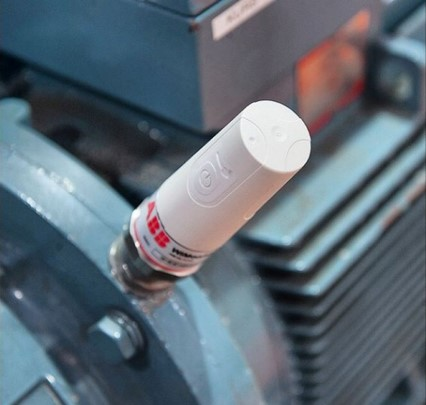
\includegraphics[width=0.6\textwidth]{INTRO/Figs/StateOfArt/abb.jpg}
        \end{figure} 
        
    \subsection{IFM VSExxx}
        IFM je německá firma se zaměřením na senzoriku v průmyslu. Přidaná hodnota produktů této společnosti tkví zejména v široké nabídce nabízených řešení. Koncový zákazník si může podle svých požadavků sestavit celý monitorovací systém. IFM nabízí různě kvalitní akcelerometry, vzorkovací obvody a monitorovací jednotky \cite{manufactor:2}. Na rozdíl od firmy ABB lze prostřednictvím dodaného softwaru VES004 konfigurovat parametry monitorování, a docílit tak různorodějších analýz. Systém nevyužívá brány, k jednotlivým jednotkám lze ale připojit více akcelerometrů. Zásadní odlišností od ostatních porovnávaných systémů je drátová komunikační infrastruktura, jejíž nasazení se příliš nehodí do již fungujících průmyslových prostředí (více v kapitole \ref{section:drat}).
        
         \begin{itemize}
            \item Konektivita: Ethernet
            \item Konfigurovatelnost: nastavitelné jsou standardní parametry monitorování
            \item Software: desktopová aplikace bez propojení s cloudem
            \item Přesnost: rozdílná podle konkrétního řešení
            \item Napájení: síťové 
            \item Cena: rozdílná podle konkrétního řešení
        \end{itemize}{}
        
        \begin{figure}[!htp]
            \centering
            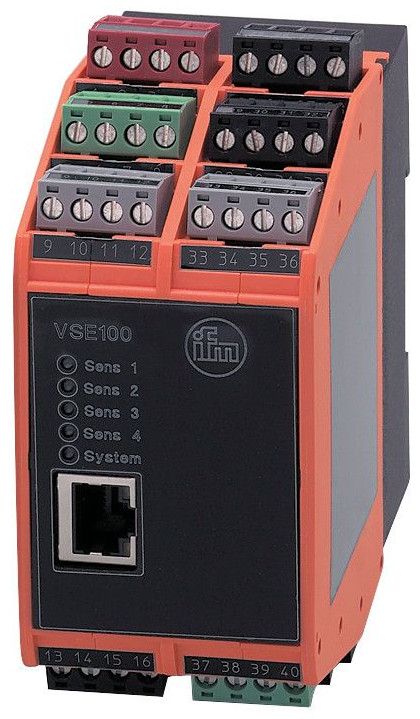
\includegraphics[width=0.25\textwidth]{INTRO/Figs/StateOfArt/ifm2.jpg}
            \caption {Jednotka VSE002 pro připojení 4 akcelerometrů. Převzato z \cite{manufactor:2}.}
        \end{figure}
        
       
        
       
       \begin{figure}[!htp]
            \centering
            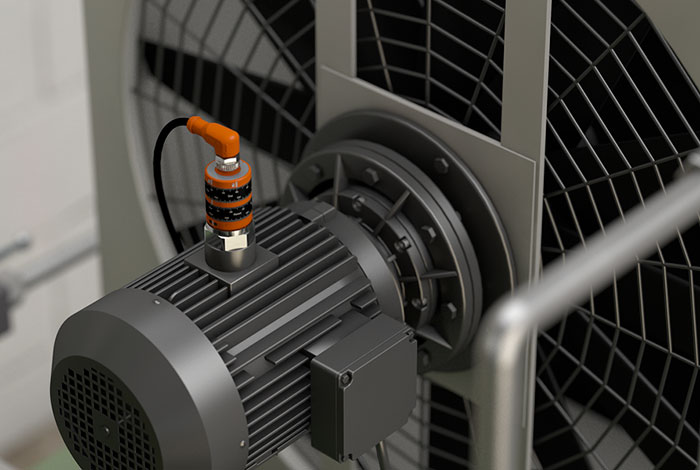
\includegraphics[width=0.7\textwidth]{INTRO/Figs/StateOfArt/ifm3.jpg}
            \caption {Upevnění akcelerometru VSE002 k motoru. Převzato z \cite{manufactor:2}.}
        \end{figure}
    
    
    \subsection{Fluke 3561 FC Vibration Sensors}
        Fluke je americká společnost zaměřující se na elektronické monitorovací a testovací systémy. Jejich produkty si na rozdíl od ABB a IFM zakládají na inovaci, a proto Fluke přináší z hlediska filosofie IIoT mnohem modernější monitorovací systém, kde vlastní diagnostika probíhá za pomocí webového klienta a mobilní aplikace. Za zmínku stojí také velmi elegantně vyřešený design, velikost a možnosti upevnění senzorů k motorům \cite{manufactor:3}.
        
     
        
        \begin{itemize}
            \item Konektivita: Low power Bluetooth 
            \item Konfigurovatelnost: pevná vzorkovací frekvence, odesílání informací do brány
            \item Software: zpracování dat prostřednictvím Fluke Connect App
            \item Přesnost: $\pm 32\,g$, šířka pásma 1 kHz
            \item Napájení: bateriové zařízení s výdrží 5 let
            \item Cena: zhruba 100 000 Kč za 4 senzory, 1 bránu a software
        \end{itemize}{}
        
          \begin{figure} [!htp]
            \centering
            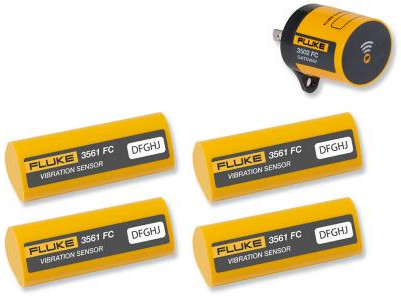
\includegraphics[width=0.4\textwidth]{INTRO/Figs/StateOfArt/fluke2.jpg}
            \caption {Brána a monitorovací jednotky Fluke. Převzato z \cite{manufactor:3}.}
        \end{figure}
    
        
        \begin{figure}[H]
            \centering
            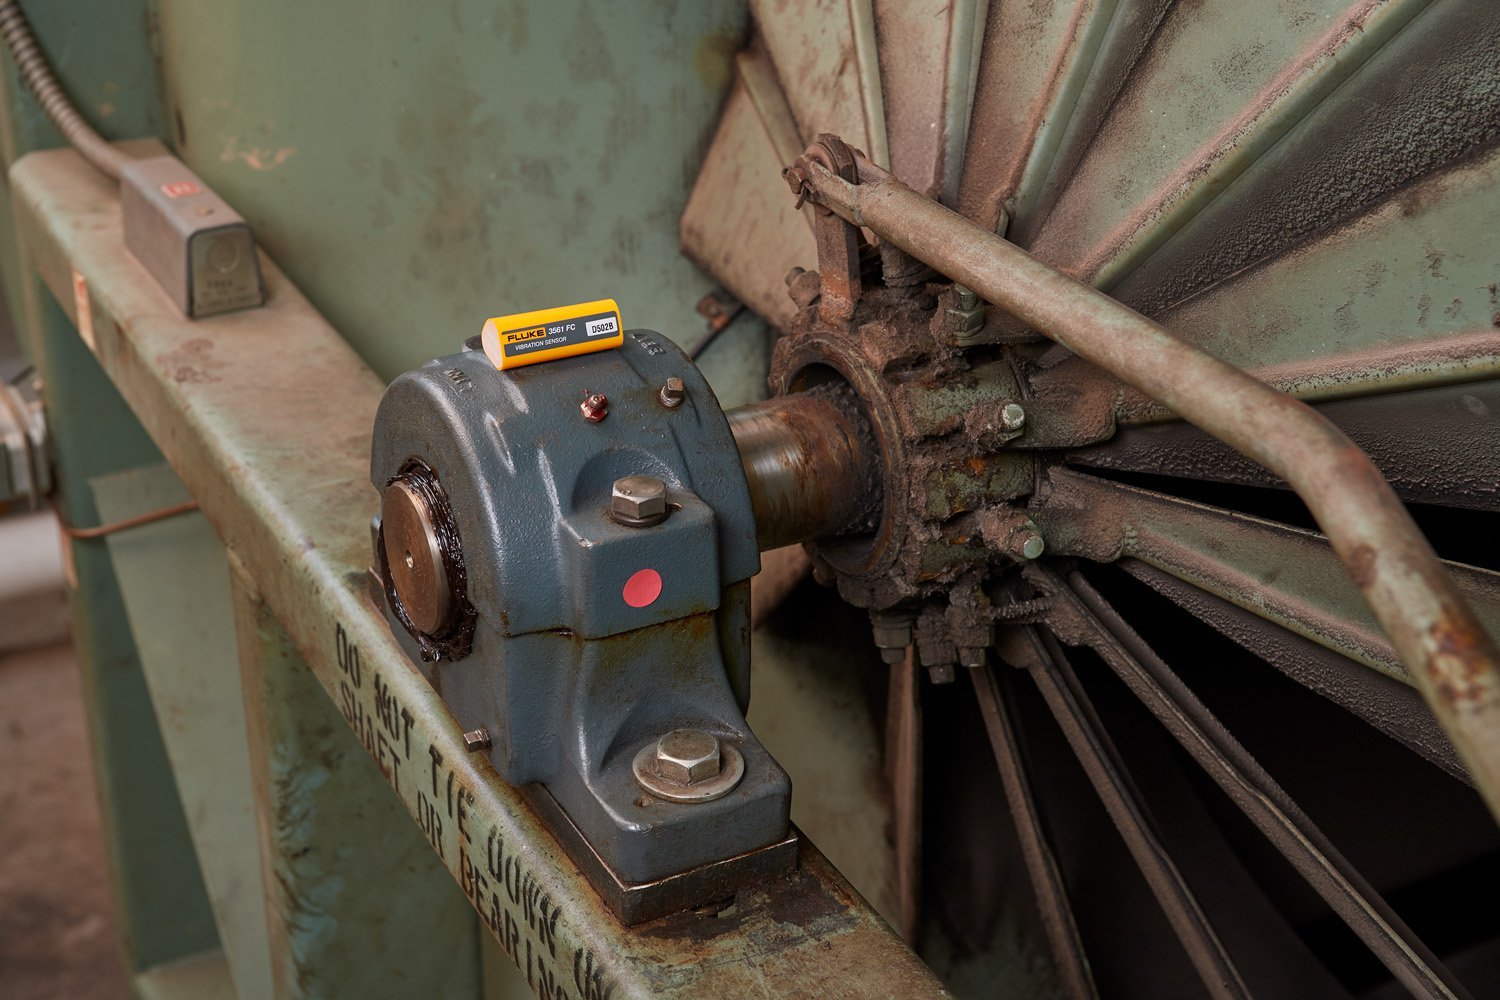
\includegraphics[width=0.75\textwidth]{INTRO/Figs/StateOfArt/fluke.jpg}
            \caption {Upevnění Fluke senzoru k motoru. Převzato z \cite{manufactor:3}.}
        \end{figure}

    
    
    \subsection{Flexs C2 Wireless Condition Analyzer}
        Společnost FlexSCADA je kanadská společnost zabývající se SCADA (Supervisory Control And Data Acquisition) systémy, tedy sběrem dat a řízením. Produkty této společnosti jsou nejflexibilnějšími, které se mi podařilo nalézt. Umožňuje především široké možnosti konfigurace monitorování (nastavení vzorkovací frekvence, počet vzorků u FFT, interval odesílání dat\ldots). Navíc přichází se zajímavým řešením, kdy po stisknutí tlačítka vytvoří zařízení hotspot, ke kterému se lze přihlásit a pozorovat současné trendy monitorování. Krom toho ale odesílá data i do cloudu ke specifičtějším analýzám \cite{manufactor:4}.\\
        Problémem jsou pouze vysoké pořizovací náklady v případě nasazení systému do velkých továren. Ačkoliv cena jednoho monitorovacího zařízení je poměrně přívětivá a najednou lze díky čtyřem akcelerometrům připojit více motorů, s~narůstajícím počtem monitorovaných zařízení cena rychle roste.
        \begin{itemize}
            \item Konektivita: WiFi, LTE
            \item Konfigurovatelnost: široká možnost konfigurace včetně parametrů monitorování
            \item Software: webový klient a aplikace + možnost odesílání dat a zpracování v cloudu
            \item Přesnost: nespecifikováno
            \item Napájení: sběr energie z elektromagnetického vyzařování, externí síťové napájení
            \item Cena: zhruba 25 000 Kč za jednotku pro maximálně čtyři motory.
        \end{itemize}{}
        
        \begin{figure} [!h]
                \centering
                \caption{FlexSCADA Condition Analyzer. Převzato z \cite{manufactor:4}.}
                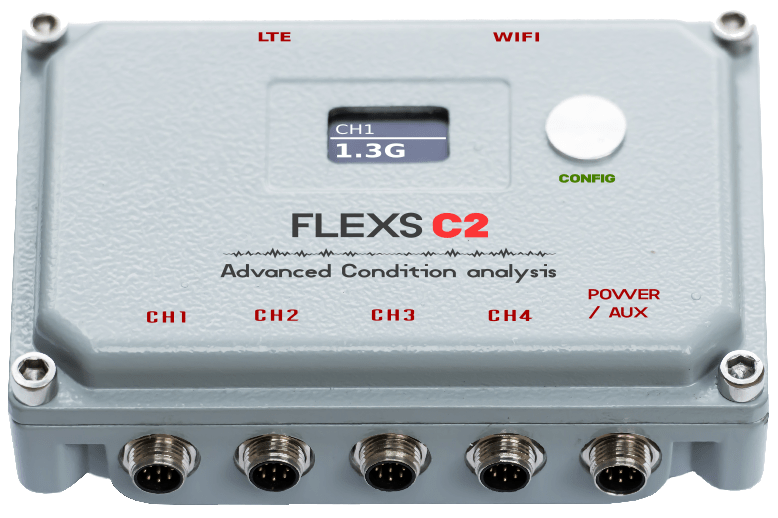
\includegraphics[width=0.7\textwidth]{INTRO/Figs/StateOfArt/flexscada.png}
        \end{figure} 


\section{Cíl práce}
    
    Cílem této práce bylo navrhnout a realizovat komplexní systém pro monitorování stavu rotačních zařízení pomocí pokročilé analýzy vibrací a teploty. Snahou bylo odlišit se od existujících řešení, vyplnit mezeru na trhu a postavit systém na základech moderních konceptů IIoT.\\
    
    \textbf{Konfigurovatelnost}
    
    Sytém se bude odlišovat od existujících zařízení na trhu zejména svoji konfigurovatelností. Uživatel bude moci pohodlně ve webovém prostředí měnit parametry monitorovací jednotky, díky čemuž bude schopen přizpůsobit zpracování monitorovaných veličin, a dosáhnout tak různorodějších a pokročilejších analýz.\\
    
    \textbf{Bezdrátová komunikace na velké vzdálenosti}
    
    Důraz bude kladen na dostupnost a univerzální použití za pomoci LPWAN sítí. Jako komunikační síť se bude využívat LoRa s velkým dosahem, nízkým datovým tokem a vysokou výdrží baterie, což umožní monitorovat stav rotačních zařízení i v případech, kdy to dříve nebylo možné (více v kapitole \ref{section:lpwan}).
    
    \textbf{Nezávislost}
    
    Systém bude také zcela nezávislý na již existujících oficiálních LoRa sítích jako The Things Network či síti Českých Radiokomunikací. Krom koncových uzlů bude tedy zahrnovat i centrální jednotku (Gateway) pro řízení komunikace s měřicími jednotkami a komunikaci s~aplikačním serverem. Tento přístup usnadňuje nasazení systému i do míst, která nejsou pokrytá signálem, nebo mají problémy s jeho silou.
    
    \textbf{Flexibilita a otevřenost}
    
   Pozornost bude věnována flexibilitě celého systému prostřednictvím použití databázového modelu a RESTového serveru, které umožní poskytnutí naměřených a vypočítaných dat aplikacím třetích stran. Díky této otevřenosti systému budou zákazníci moci data zpracovávat podle svých požadavků a snadněji je integrovat do vlastních systémů.
   
   \textbf{Cena}
   
   Vzhledem k tomu, že produkt je studentskou prací, cena celého systému bude tlačena co možná nejníže.
   
%CHECK ~
%CHECK red
%CHECK ...